%% bare_jrnl.tex
%% V1.4
%% 2012/12/27
%% by Michael Shell
%% see http://www.michaelshell.org/
%% for current contact information.
%%
%% This is a skeleton file demonstrating the use of IEEEtran.cls
%% (requires IEEEtran.cls version 1.8 or later) with an IEEE journal paper.
%%
%% Support sites:
%% http://www.michaelshell.org/tex/ieeetran/
%% http://www.ctan.org/tex-archive/macros/latex/contrib/IEEEtran/
%% and
%% http://www.ieee.org/



% *** Authors should verify (and, if needed, correct) their LaTeX system  ***
% *** with the testflow diagnostic prior to trusting their LaTeX platform ***
% *** with production work. IEEE's font choices can trigger bugs that do  ***
% *** not appear when using other class files.                            ***
% The testflow support page is at:
% http://www.michaelshell.org/tex/testflow/


%%*************************************************************************
%% Legal Notice:
%% This code is offered as-is without any warranty either expressed or
%% implied; without even the implied warranty of MERCHANTABILITY or
%% FITNESS FOR A PARTICULAR PURPOSE! 
%% User assumes all risk.
%% In no event shall IEEE or any contributor to this code be liable for
%% any damages or losses, including, but not limited to, incidental,
%% consequential, or any other damages, resulting from the use or misuse
%% of any information contained here.
%%
%% All comments are the opinions of their respective authors and are not
%% necessarily endorsed by the IEEE.
%%
%% This work is distributed under the LaTeX Project Public License (LPPL)
%% ( http://www.latex-project.org/ ) version 1.3, and may be freely used,
%% distributed and modified. A copy of the LPPL, version 1.3, is included
%% in the base LaTeX documentation of all distributions of LaTeX released
%% 2003/12/01 or later.
%% Retain all contribution notices and credits.
%% ** Modified files should be clearly indicated as such, including  **
%% ** renaming them and changing author support contact information. **
%%
%% File list of work: IEEEtran.cls, IEEEtran_HOWTO.pdf, bare_adv.tex,
%%                    bare_conf.tex, bare_jrnl.tex, bare_jrnl_compsoc.tex,
%%                    bare_jrnl_transmag.tex
%%*************************************************************************

% Note that the a4paper option is mainly intended so that authors in
% countries using A4 can easily print to A4 and see how their papers will
% look in print - the typesetting of the document will not typically be
% affected with changes in paper size (but the bottom and side margins will).
% Use the testflow package mentioned above to verify correct handling of
% both paper sizes by the user's LaTeX system.
%
% Also note that the "draftcls" or "draftclsnofoot", not "draft", option
% should be used if it is desired that the figures are to be displayed in
% draft mode.
%
\documentclass[journal]{IEEEtran}
\usepackage{graphicx}
\bibliographystyle{IEEEtran}
\usepackage{indentfirst}
%
% If IEEEtran.cls has not been installed into the LaTeX system files,
% manually specify the path to it like:
% \documentclass[journal]{../sty/IEEEtran}





% Some very useful LaTeX packages include:
% (uncomment the ones you want to load)


% *** MISC UTILITY PACKAGES ***
%
%\usepackage{ifpdf}
% Heiko Oberdiek's ifpdf.sty is very useful if you need conditional
% compilation based on whether the output is pdf or dvi.
% usage:
% \ifpdf
%   % pdf code
% \else
%   % dvi code
% \fi
% The latest version of ifpdf.sty can be obtained from:
% http://www.ctan.org/tex-archive/macros/latex/contrib/oberdiek/
% Also, note that IEEEtran.cls V1.7 and later provides a builtin
% \ifCLASSINFOpdf conditional that works the same way.
% When switching from latex to pdflatex and vice-versa, the compiler may
% have to be run twice to clear warning/error messages.






% *** CITATION PACKAGES ***
%
%\usepackage{cite}
% cite.sty was written by Donald Arseneau
% V1.6 and later of IEEEtran pre-defines the format of the cite.sty package
% \cite{} output to follow that of IEEE. Loading the cite package will
% result in citation numbers being automatically sorted and properly
% "compressed/ranged". e.g., [1], [9], [2], [7], [5], [6] without using
% cite.sty will become [1], [2], [5]--[7], [9] using cite.sty. cite.sty's
% \cite will automatically add leading space, if needed. Use cite.sty's
% noadjust option (cite.sty V3.8 and later) if you want to turn this off
% such as if a citation ever needs to be enclosed in parenthesis.
% cite.sty is already installed on most LaTeX systems. Be sure and use
% version 4.0 (2003-05-27) and later if using hyperref.sty. cite.sty does
% not currently provide for hyperlinked citations.
% The latest version can be obtained at:
% http://www.ctan.org/tex-archive/macros/latex/contrib/cite/
% The documentation is contained in the cite.sty file itself.






% *** GRAPHICS RELATED PACKAGES ***
%
\ifCLASSINFOpdf
  % \usepackage[pdftex]{graphicx}
  % declare the path(s) where your graphic files are
  % \graphicspath{{../pdf/}{../jpeg/}}
  % and their extensions so you won't have to specify these with
  % every instance of \includegraphics
  % \DeclareGraphicsExtensions{.pdf,.jpeg,.png}
\else
  % or other class option (dvipsone, dvipdf, if not using dvips). graphicx
  % will default to the driver specified in the system graphics.cfg if no
  % driver is specified.
  % \usepackage[dvips]{graphicx}
  % declare the path(s) where your graphic files are
  % \graphicspath{{../eps/}}
  % and their extensions so you won't have to specify these with
  % every instance of \includegraphics
  % \DeclareGraphicsExtensions{.eps}
\fi
% graphicx was written by David Carlisle and Sebastian Rahtz. It is
% required if you want graphics, photos, etc. graphicx.sty is already
% installed on most LaTeX systems. The latest version and documentation
% can be obtained at: 
% http://www.ctan.org/tex-archive/macros/latex/required/graphics/
% Another good source of documentation is "Using Imported Graphics in
% LaTeX2e" by Keith Reckdahl which can be found at:
% http://www.ctan.org/tex-archive/info/epslatex/
%
% latex, and pdflatex in dvi mode, support graphics in encapsulated
% postscript (.eps) format. pdflatex in pdf mode supports graphics
% in .pdf, .jpeg, .png and .mps (metapost) formats. Users should ensure
% that all non-photo figures use a vector format (.eps, .pdf, .mps) and
% not a bitmapped formats (.jpeg, .png). IEEE frowns on bitmapped formats
% which can result in "jaggedy"/blurry rendering of lines and letters as
% well as large increases in file sizes.
%
% You can find documentation about the pdfTeX application at:
% http://www.tug.org/applications/pdftex





% *** MATH PACKAGES ***
%
%\usepackage[cmex10]{amsmath}
% A popular package from the American Mathematical Society that provides
% many useful and powerful commands for dealing with mathematics. If using
% it, be sure to load this package with the cmex10 option to ensure that
% only type 1 fonts will utilized at all point sizes. Without this option,
% it is possible that some math symbols, particularly those within
% footnotes, will be rendered in bitmap form which will result in a
% document that can not be IEEE Xplore compliant!
%
% Also, note that the amsmath package sets \interdisplaylinepenalty to 10000
% thus preventing page breaks from occurring within multiline equations. Use:
%\interdisplaylinepenalty=2500
% after loading amsmath to restore such page breaks as IEEEtran.cls normally
% does. amsmath.sty is already installed on most LaTeX systems. The latest
% version and documentation can be obtained at:
% http://www.ctan.org/tex-archive/macros/latex/required/amslatex/math/





% *** SPECIALIZED LIST PACKAGES ***
%
%\usepackage{algorithmic}
% algorithmic.sty was written by Peter Williams and Rogerio Brito.
% This package provides an algorithmic environment fo describing algorithms.
% You can use the algorithmic environment in-text or within a figure
% environment to provide for a floating algorithm. Do NOT use the algorithm
% floating environment provided by algorithm.sty (by the same authors) or
% algorithm2e.sty (by Christophe Fiorio) as IEEE does not use dedicated
% algorithm float types and packages that provide these will not provide
% correct IEEE style captions. The latest version and documentation of
% algorithmic.sty can be obtained at:
% http://www.ctan.org/tex-archive/macros/latex/contrib/algorithms/
% There is also a support site at:
% http://algorithms.berlios.de/index.html
% Also of interest may be the (relatively newer and more customizable)
% algorithmicx.sty package by Szasz Janos:
% http://www.ctan.org/tex-archive/macros/latex/contrib/algorithmicx/




% *** ALIGNMENT PACKAGES ***
%
%\usepackage{array}
% Frank Mittelbach's and David Carlisle's array.sty patches and improves
% the standard LaTeX2e array and tabular environments to provide better
% appearance and additional user controls. As the default LaTeX2e table
% generation code is lacking to the point of almost being broken with
% respect to the quality of the end results, all users are strongly
% advised to use an enhanced (at the very least that provided by array.sty)
% set of table tools. array.sty is already installed on most systems. The
% latest version and documentation can be obtained at:
% http://www.ctan.org/tex-archive/macros/latex/required/tools/


% IEEEtran contains the IEEEeqnarray family of commands that can be used to
% generate multiline equations as well as matrices, tables, etc., of high
% quality.




% *** SUBFIGURE PACKAGES ***
%\ifCLASSOPTIONcompsoc
%  \usepackage[caption=false,font=normalsize,labelfont=sf,textfont=sf]{subfig}
%\else
%  \usepackage[caption=false,font=footnotesize]{subfig}
%\fi
% subfig.sty, written by Steven Douglas Cochran, is the modern replacement
% for subfigure.sty, the latter of which is no longer maintained and is
% incompatible with some LaTeX packages including fixltx2e. However,
% subfig.sty requires and automatically loads Axel Sommerfeldt's caption.sty
% which will override IEEEtran.cls' handling of captions and this will result
% in non-IEEE style figure/table captions. To prevent this problem, be sure
% and invoke subfig.sty's "caption=false" package option (available since
% subfig.sty version 1.3, 2005/06/28) as this is will preserve IEEEtran.cls
% handling of captions.
% Note that the Computer Society format requires a larger sans serif font
% than the serif footnote size font used in traditional IEEE formatting
% and thus the need to invoke different subfig.sty package options depending
% on whether compsoc mode has been enabled.
%
% The latest version and documentation of subfig.sty can be obtained at:
% http://www.ctan.org/tex-archive/macros/latex/contrib/subfig/




% *** FLOAT PACKAGES ***
%
%\usepackage{fixltx2e}
% fixltx2e, the successor to the earlier fix2col.sty, was written by
% Frank Mittelbach and David Carlisle. This package corrects a few problems
% in the LaTeX2e kernel, the most notable of which is that in current
% LaTeX2e releases, the ordering of single and double column floats is not
% guaranteed to be preserved. Thus, an unpatched LaTeX2e can allow a
% single column figure to be placed prior to an earlier double column
% figure. The latest version and documentation can be found at:
% http://www.ctan.org/tex-archive/macros/latex/base/


%\usepackage{stfloats}
% stfloats.sty was written by Sigitas Tolusis. This package gives LaTeX2e
% the ability to do double column floats at the bottom of the page as well
% as the top. (e.g., "\begin{figure*}[!b]" is not normally possible in
% LaTeX2e). It also provides a command:
%\fnbelowfloat
% to enable the placement of footnotes below bottom floats (the standard
% LaTeX2e kernel puts them above bottom floats). This is an invasive package
% which rewrites many portions of the LaTeX2e float routines. It may not work
% with other packages that modify the LaTeX2e float routines. The latest
% version and documentation can be obtained at:
% http://www.ctan.org/tex-archive/macros/latex/contrib/sttools/
% Do not use the stfloats baselinefloat ability as IEEE does not allow
% \baselineskip to stretch. Authors submitting work to the IEEE should note
% that IEEE rarely uses double column equations and that authors should try
% to avoid such use. Do not be tempted to use the cuted.sty or midfloat.sty
% packages (also by Sigitas Tolusis) as IEEE does not format its papers in
% such ways.
% Do not attempt to use stfloats with fixltx2e as they are incompatible.
% Instead, use Morten Hogholm'a dblfloatfix which combines the features
% of both fixltx2e and stfloats:
%
% \usepackage{dblfloatfix}
% The latest version can be found at:
% http://www.ctan.org/tex-archive/macros/latex/contrib/dblfloatfix/




%\ifCLASSOPTIONcaptionsoff
%  \usepackage[nomarkers]{endfloat}
% \let\MYoriglatexcaption\caption
% \renewcommand{\caption}[2][\relax]{\MYoriglatexcaption[#2]{#2}}
%\fi
% endfloat.sty was written by James Darrell McCauley, Jeff Goldberg and 
% Axel Sommerfeldt. This package may be useful when used in conjunction with 
% IEEEtran.cls'  captionsoff option. Some IEEE journals/societies require that
% submissions have lists of figures/tables at the end of the paper and that
% figures/tables without any captions are placed on a page by themselves at
% the end of the document. If needed, the draftcls IEEEtran class option or
% \CLASSINPUTbaselinestretch interface can be used to increase the line
% spacing as well. Be sure and use the nomarkers option of endfloat to
% prevent endfloat from "marking" where the figures would have been placed
% in the text. The two hack lines of code above are a slight modification of
% that suggested by in the endfloat docs (section 8.4.1) to ensure that
% the full captions always appear in the list of figures/tables - even if
% the user used the short optional argument of \caption[]{}.
% IEEE papers do not typically make use of \caption[]'s optional argument,
% so this should not be an issue. A similar trick can be used to disable
% captions of packages such as subfig.sty that lack options to turn off
% the subcaptions:
% For subfig.sty:
% \let\MYorigsubfloat\subfloat
% \renewcommand{\subfloat}[2][\relax]{\MYorigsubfloat[]{#2}}
% However, the above trick will not work if both optional arguments of
% the \subfloat command are used. Furthermore, there needs to be a
% description of each subfigure *somewhere* and endfloat does not add
% subfigure captions to its list of figures. Thus, the best approach is to
% avoid the use of subfigure captions (many IEEE journals avoid them anyway)
% and instead reference/explain all the subfigures within the main caption.
% The latest version of endfloat.sty and its documentation can obtained at:
% http://www.ctan.org/tex-archive/macros/latex/contrib/endfloat/
%
% The IEEEtran \ifCLASSOPTIONcaptionsoff conditional can also be used
% later in the document, say, to conditionally put the References on a 
% page by themselves.




% *** PDF, URL AND HYPERLINK PACKAGES ***
%
%\usepackage{url}
% url.sty was written by Donald Arseneau. It provides better support for
% handling and breaking URLs. url.sty is already installed on most LaTeX
% systems. The latest version and documentation can be obtained at:
% http://www.ctan.org/tex-archive/macros/latex/contrib/url/
% Basically, \url{my_url_here}.




% *** Do not adjust lengths that control margins, column widths, etc. ***
% *** Do not use packages that alter fonts (such as pslatex).         ***
% There should be no need to do such things with IEEEtran.cls V1.6 and later.
% (Unless specifically asked to do so by the journal or conference you plan
% to submit to, of course. )


% correct bad hyphenation here
\hyphenation{op-tical net-works semi-conduc-tor}


\begin{document}
%
% paper title
% can use linebreaks \\ within to get better formatting as desired
% Do not put math or special symbols in the title.
\title{A Survey on Distributed Computation Frameworks}
%
%
% author names and IEEE memberships
% note positions of commas and nonbreaking spaces ( ~ ) LaTeX will not break
% a structure at a ~ so this keeps an author's name from being broken across
% two lines.
% use \thanks{} to gain access to the first footnote area
% a separate \thanks must be used for each paragraph as LaTeX2e's \thanks
% was not built to handle multiple paragraphs
%

\author{Yongbin Liu, Yanqiong Hu, Haiyan Liu, Funan Zhou}

% note the % following the last \IEEEmembership and also \thanks - 
% these prevent an unwanted space from occurring between the last author name
% and the end of the author line. i.e., if you had this:
% 
% \author{....lastname \thanks{...} \thanks{...} }
%                     ^------------^------------^----Do not want these spaces!
%
% a space would be appended to the last name and could cause every name on that
% line to be shifted left slightly. This is one of those "LaTeX things". For
% instance, "\textbf{A} \textbf{B}" will typeset as "A B" not "AB". To get
% "AB" then you have to do: "\textbf{A}\textbf{B}"
% \thanks is no different in this regard, so shield the last } of each \thanks
% that ends a line with a % and do not let a space in before the next \thanks.
% Spaces after \IEEEmembership other than the last one are OK (and needed) as
% you are supposed to have spaces between the names. For what it is worth,
% this is a minor point as most people would not even notice if the said evil
% space somehow managed to creep in.



% The paper headers
\markboth{Journal of \LaTeX\ Class Files,~Vol.~11, No.~4, December~2012}%
{Shell \MakeLowercase{\textit{et al.}}: Bare Demo of IEEEtran.cls for Journals}
% The only time the second header will appear is for the odd numbered pages
% after the title page when using the twoside option.
% 
% *** Note that you probably will NOT want to include the author's ***
% *** name in the headers of peer review papers.                   ***
% You can use \ifCLASSOPTIONpeerreview for conditional compilation here if
% you desire.




% If you want to put a publisher's ID mark on the page you can do it like
% this:
%\IEEEpubid{0000--0000/00\$00.00~\copyright~2012 IEEE}
% Remember, if you use this you must call \IEEEpubidadjcol in the second
% column for its text to clear the IEEEpubid mark.



% use for special paper notices
%\IEEEspecialpapernotice{(Invited Paper)}




% make the title area
\maketitle

% As a general rule, do not put math, special symbols or citations
% in the abstract or keywords.
\begin{abstract}
The abstract goes here.
\end{abstract}

% Note that keywords are not normally used for peerreview papers.
\begin{IEEEkeywords}
IEEEtran, journal, \LaTeX, paper, template.
\end{IEEEkeywords}






% For peer review papers, you can put extra information on the cover
% page as needed:
% \ifCLASSOPTIONpeerreview
% \begin{center} \bfseries EDICS Category: 3-BBND \end{center}
% \fi
%
% For peerreview papers, this IEEEtran command inserts a page break and
% creates the second title. It will be ignored for other modes.
\IEEEpeerreviewmaketitle



\section{Introduction}
% The very first letter is a 2 line initial drop letter followed
% by the rest of the first word in caps.
% 
% form to use if the first word consists of a single letter:
% \IEEEPARstart{A}{demo} file is ....
% 
% form to use if you need the single drop letter followed by
% normal text (unknown if ever used by IEEE):
% \IEEEPARstart{A}{}demo file is ....
% 
% Some journals put the first two words in caps:
% \IEEEPARstart{T}{his demo} file is ....
% 
% Here we have the typical use of a "T" for an initial drop letter
% and "HIS" in caps to complete the first word.
\IEEEPARstart{T}{his} demo file is intended to serve as a ``starter file''
for IEEE journal papers produced under \LaTeX\ using
IEEEtran.cls version 1.8 and later.
% You must have at least 2 lines in the paragraph with the drop letter
% (should never be an issue)
I wish you the best of success.

\hfill mds
 
\hfill December 27, 2012

\subsection{Subsection Heading Here}
Subsection text here.

% needed in second column of first page if using \IEEEpubid
%\IEEEpubidadjcol

\subsubsection{Subsubsection Heading Here}
Subsubsection text here.


% An example of a floating figure using the graphicx package.
% Note that \label must occur AFTER (or within) \caption.
% For figures, \caption should occur after the \includegraphics.
% Note that IEEEtran v1.7 and later has special internal code that
% is designed to preserve the operation of \label within \caption
% even when the captionsoff option is in effect. However, because
% of issues like this, it may be the safest practice to put all your
% \label just after \caption rather than within \caption{}.
%
% Reminder: the "draftcls" or "draftclsnofoot", not "draft", class
% option should be used if it is desired that the figures are to be
% displayed while in draft mode.
%
%\begin{figure}[!t]
%\centering
%\includegraphics[width=2.5in]{myfigure}
% where an .eps filename suffix will be assumed under latex, 
% and a .pdf suffix will be assumed for pdflatex; or what has been declared
% via \DeclareGraphicsExtensions.
%\caption{Simulation Results.}
%\label{fig_sim}
%\end{figure}

% Note that IEEE typically puts floats only at the top, even when this
% results in a large percentage of a column being occupied by floats.


% An example of a double column floating figure using two subfigures.
% (The subfig.sty package must be loaded for this to work.)
% The subfigure \label commands are set within each subfloat command,
% and the \label for the overall figure must come after \caption.
% \hfil is used as a separator to get equal spacing.
% Watch out that the combined width of all the subfigures on a 
% line do not exceed the text width or a line break will occur.
%
%\begin{figure*}[!t]
%\centering
%\subfloat[Case I]{\includegraphics[width=2.5in]{box}%
%\label{fig_first_case}}
%\hfil
%\subfloat[Case II]{\includegraphics[width=2.5in]{box}%
%\label{fig_second_case}}
%\caption{Simulation results.}
%\label{fig_sim}
%\end{figure*}
%
% Note that often IEEE papers with subfigures do not employ subfigure
% captions (using the optional argument to \subfloat[]), but instead will
% reference/describe all of them (a), (b), etc., within the main caption.


% An example of a floating table. Note that, for IEEE style tables, the 
% \caption command should come BEFORE the table. Table text will default to
% \footnotesize as IEEE normally uses this smaller font for tables.
% The \label must come after \caption as always.
%
%\begin{table}[!t]
%% increase table row spacing, adjust to taste
%\renewcommand{\arraystretch}{1.3}
% if using array.sty, it might be a good idea to tweak the value of
% \extrarowheight as needed to properly center the text within the cells
%\caption{An Example of a Table}
%\label{table_example}
%\centering
%% Some packages, such as MDW tools, offer better commands for making tables
%% than the plain LaTeX2e tabular which is used here.
%\begin{tabular}{|c||c|}
%\hline
%One & Two\\
%\hline
%Three & Four\\
%\hline
%\end{tabular}
%\end{table}


% Note that IEEE does not put floats in the very first column - or typically
% anywhere on the first page for that matter. Also, in-text middle ("here")
% positioning is not used. Most IEEE journals use top floats exclusively.
% Note that, LaTeX2e, unlike IEEE journals, places footnotes above bottom
% floats. This can be corrected via the \fnbelowfloat command of the
% stfloats package.

\section{Map-Reduce Like Frameworks}

With the expansion of Google search service and the increase of data volume, many applications need more than one machine to compute in parallel, so the MPI framework is proposed. However, the traditional MPI framework code is complex and has no fault tolerance mechanism. The MapReduce framework was proposed, which makes up for the defects of MPI. With the application of large-scale distributed machine learning, MapReduce involves a large number of unnecessary disk reads and writes, so Spark model is proposed. Because MapReduce model is relatively fixed, a Dryad model that can customize DAG graph is proposed.
% needed in second column of first page if using \IEEEpubid
%\IEEEpubidadjcol
\subsection{Mapreduce model}

The MapReduce\cite{MapReduce} framework consists of map and reduce.From the figure \ref{figure1},The system automatically divides the input file into M blocks, and the map workpoint calls blocks to run on multiple computers. The intermediate key/value pairs generated by the map function are divided into R blocks, which are called by the reduce workpoint.Map and reduce nodes are both invoked through the master node.

For example,we count the number of words that appear in a large number of documents.In this problem,key is a word and value is set to 1.The map function simply outputs key/value pairs.The reduce function sums together all counts emitted for a particular word.

%map(String key, String value): 

%for each word w in value:

%EmitIntermediate(w, "1"); 

%reduce(String key, Iterator values): 

%int result = 0; 

%for each v in values: 

%result += ParseInt(v); 

%Emit(AsString(result)); 

MapReduce framework has a good fault-tolerant mechanism. When the work node does not respond, the work node is marked as failing. Its map or reduce tasks can be scheduled by other nodes. When the primary node fails, the MapReduce computation needs to be terminated and the MapReduce operation restarted. However, MapReduce is inefficient in the application of iterative algorithms and interactive data mining tools, and its model is relatively fixed and inflexible.
\begin{figure}
	\centering
	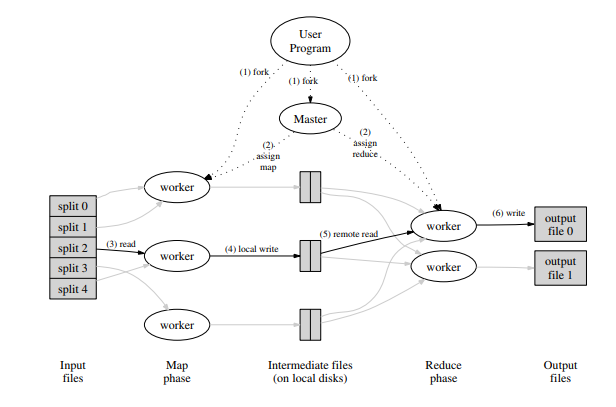
\includegraphics[width = 0.4\textwidth]{1.png}
	\caption{Execution overview}
	\label{figure1}
\end{figure} 

\subsection{Spark}
Spark framework\cite{Spark} is more efficient in solving such problems as iterative algorithms and interactive data mining tools.

The Spark framework is composed of RDD\cite{RDD} and some parallel operations.On Spark, RDD is represented as objects that are converted by calling methods (or functions) on those objects. RDD provides a highly constrained Shared memory model in which RDD is a collection of read-only record partitions that can only be created by performing certain transformations on other RDD,Such as map, filter and so on.

For example, the operator identifies the cause of the error from  the HDFS of the error site.
%Using Spark, the operator simply loads the error information in the log into the memory of a set of nodes and then performs an interactive query.

lines = spark.textFile("hdfs://...")

errors = lines.filter(.startsWith("ERROR"))

errors.cache()

Errors. The filter (.The contains (" MySQL ")).The count ()

Errors. The filter (.The contains (" HDFS "))

The map (.The split (' \  t ') )

Collect ()

In picture \ref{figure2}, the program defines an RDD (text line set) from the HDFS file, and the error obtained after filter operation is cached in the memory, and then the new RDD is obtained after filter and map operation, and finally the RDD is collected operation.			

Spark implements Shared memory through RDD.RDD also has fault-tolerant mechanisms. If a partition is lost, it can be rebuilt. But RDD has limitations.RDDs can not write fine-grained data.So It is only suitable for iterative computing applications.
%Since the Spark framework is supported by Scala, the memory management of Java Virtual Machine seems still a problem.
\subsection{Dryad}
Dryad framework\cite{Dryad} make programming more flexible. Dryad is suitable for cloud computing or program related to directed acyclic graphs.
\begin{figure}
	\begin{center}
		\begin{minipage}[c]{0.25\textwidth}
			\centering
			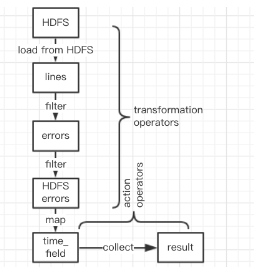
\includegraphics[width = 1\textwidth]{2.png}
			\centering
			\caption{Implementation overview}
			\label{figure2}
		\end{minipage}%
		\begin{minipage}[c]{0.25\textwidth} 
			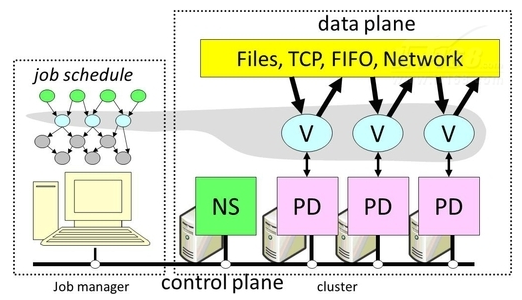
\includegraphics[width = 1\textwidth]{4.png}
			\caption{Dryad system structure.Each node in the figure represents a program to be executed, and the edges between nodes represent the transmission mode of data in the data channel, which may be files, TCP Pipe, Shared memory, etc.}
			\label{figure3}
		\end{minipage}
	\end{center}
\end{figure} 

Dryad's system is generally built to support parallel programs with Directed Acycline Graph (DAG) type data flows.In figure \ref{figure3}, we build our own directed acyclic graph, the task manager (JM) gets the graph, gets the list of available computers through the named server (NS), and schedules the program through a maintenance process (PD).
\begin{figure}
	\centering
	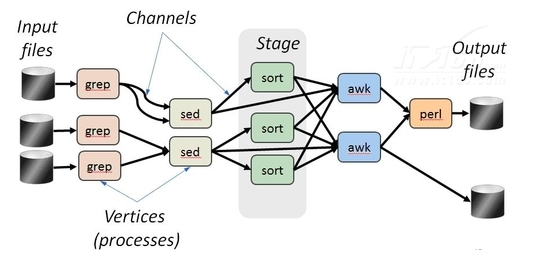
\includegraphics[width = 0.3\textwidth]{5.png}
	\centering
	\caption{Task structure of Dryad }
	\label{levfig}
\end{figure} 

In the figure \ref{levfig},We find that Dryad's execution process is very similar to MapReduce, except that MapReduce is a map and reduce phase, while Dryad is always invoked through Vertexs.

Dryad is one of the key technologies to implement and build Microsoft's cloud computing infrastructure. Dryad is flexible enough to write and modify DAG diagrams to suit your needs.
however, Dryad has limitations. It is more suitable for batch tasks than for tasks requiring quick response; This data model is more suitable for processing stream access than random access.


\section{Graph Model}
Many practical computing problems concern large graphs, e.g., the Web graph and social networks. While MapReduce is ill-suited for graph prcessing since many iterations are needed for parallel graph processing and materializations of intermediate results at every MapReduce iteration harm performance. In the following, we briefly describe three classical graph computation model.

\subsection{Pregel abstraction}
In Pregel\cite{Pregel}, programs are expressed as a sequence of iterations called supersteps which is inspired by Bulk Synchronous Parallel model(BSP). Fig. \ref{pregel} illustrates an abstract model of a sequence of supersteps used in Pregel. The vertices compute in parallel within each superstep. Each vertax reads messages sent to itself in previous superstep and executes the same user-defined function, then it can send messages to its neighbors in the next superstep, or mutate the topology of the graph. A vertex will vote to halt if it has no further work to do and algorithm termination is based on every vertex voting to halt. The vertex-centric approach is flexible and easy to deliver to users.
\begin{figure}
	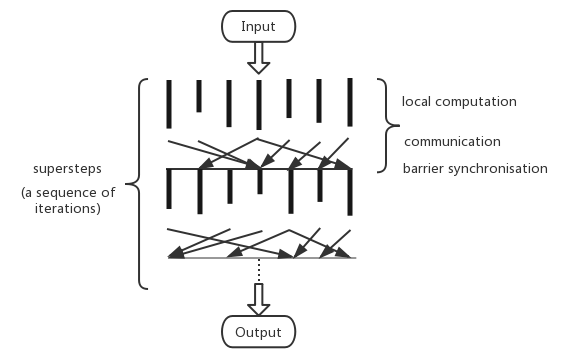
\includegraphics[width=\linewidth]{pregel.jpg}
	\caption{a model of superstep processing}
	\label{pregel}
\end{figure}

The performance, scalability and fault-tolerance of Pregel have already been satisfactory for graphs with billions of vertices\cite{Pregel}. There still has some work to do like avoiding the cost of faster workers having to wait frequently at inter-superstep barriers.
\subsection{GraphLab abstraction}
By targeting common patterns in ML like sparse data dependencies and asynchronous iterative computation, GraphLab presents an asynchronous distributed shared-memory framework in which vertex-programs share access to a distributed graph with data stored on every vertex and edge.

GraphLab provides a choice of three data consistency models which enable the user to balance performance and data consistency. And it also provides an asynchronous computation model in which vertex-programs can schedule neighboring vertex-programs to be executed in the future. The dynamic scheduling can reduce the performance degradation of load imbalance problem which exists in Pregel\cite{Pregel}.

GraphLab supports the representation of structured data dependencies, iterative computation, and flexible scheduling. While the process of extending the GraphLab framework to the distributed setting faces some new challenges including efficient graph partitioning, loading balancing, distributed locking and fault tolerance\cite{GraphLab}. 
\subsection{PowerGraph abstraction}
Graphs derived from real world often exhibit power-law degree distributions, which are difficult to partition and can lead to work imbalance and increasing communication and storage. Both Pregel and GaphLab place a graph on a cluster by edge-cuts which perform poorly on power-law graphs.

PowerGraph eliminates the degree dependence of the vertex-program by directly exploiting the GAS decomposition to factor vertex-programs over edges\cite{PowerGraph}. The GAS model represents three conceptual phases of a vertex-program: Gather, Apply, and Scatter. Fig. \ref{powergraph1} is an example of the PageRank program implemented in PowerGraph\cite{PageRank}.
\begin{figure}
	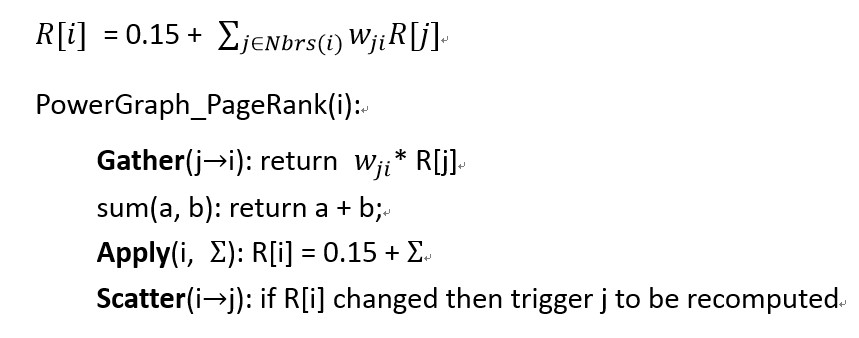
\includegraphics[width=\linewidth]{powergraph1.jpg}
	\caption{PageRank vertex-program implemented in PowerGraph}
	\label{powergraph1}
\end{figure}
\begin{figure}
	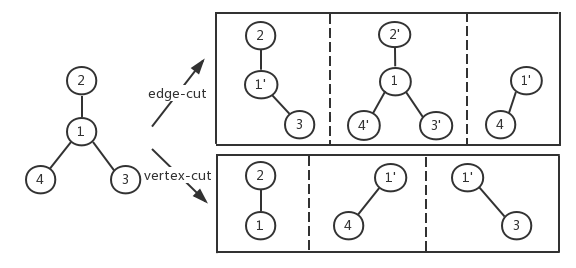
\includegraphics[width=\linewidth]{powergraph2.jpg}
	\caption{an example of edge-cut and vertex-cut of a graph into three parts}
	\label{powergraph2}
\end{figure}

Because GraphLab and Pregel use edge-cuts, their communication volume is proportional to the number of ghosts: the replicated vertex and edge data along the partition boundary. In Fig. \ref{powergraph2} we construct a three-way cut of a four vertex graph: edge-cut requires more communication with five ghost vertices and all edge data being replicated while vertex-cut only results in two ghost vertices. When using a vertex-cut, gather function runs locally on each machine and then the result of sum is sent from each mirror to the master. The master runs the apply function to update vertex data and then sends the new information to all mirrors. Finally the scatter phase is run in parallel on mirrors to update the data on adjacent edges\cite{PowerGraph}.

PowerGraph’s total computation volume and runtime of one iteration of PageRank on the Twitter follower graph is much less than Pregel and GraphLab. As a consequence, PowerGraph is robust to high-degree vertices.

\section{State-Based Distributed Computation Frameworks}
With the boom of large scale deep artificial convolutional networks, great demands for large distributed training systems emerged. The training process of most machine learning algorithms come down to gradient descent methods. During each iteration, parameters of machine learning models are updated. When the scale of dataset is very large, the computation of gradients are distributed across multiple hosts. The traditional frameworks like Map-Reduce and Spark mainly train machine learning models with synchronous iterative steps. In each step, the gradients are computed across different servers and then get average gradients. The new gradients are updated to all servers and new iterations start. 

However, the efficiency of these frameworks is limited owing to the synchronous iterative mechanism. The execution time of each step is determined by the slowest server which is called \textit{straggler}. These kinds of models obey the bulk synchronous parallel (BSP) \cite{valiant1990bridging} framework. Another trial was proposed that all the parallel workers in a cluster do their own tasks and update parameters by themselves which is called asynchronous parallel model. However, it's difficult to ensure the gradients to converge since the parameters of all of the workers are not consistent. As a trade-off between high-performance and gradient convergence, a new protocol called staleness synchronous parallel was utilized. It allows users to define a threshold to coordinate the steps of all workers. Only if the iteration counts of all workers do not exceed the threshold, the training process will continue, otherwise the faster workers will stop to wait for the stragglers.

\begin{figure}
    \centering
    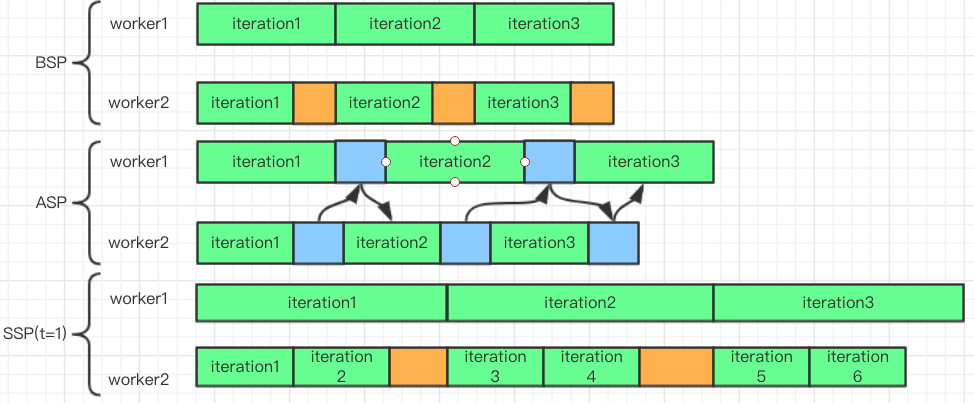
\includegraphics[height=0.3\textwidth, width=\linewidth]{SSP_ASP_BSP.png}
    \caption{The comparison of three data parallel models, in which the green grids demonstrate the computation time interval and the orange ones indicate an idle time interval. During the blue time interval, workers communicate to share parameters.}
    \label{fig:my_label}
\end{figure}

All of the shared parameters and dependency in the large-scale machine learning systems are stored using distributed in-memory database and fault-tolerance mechanism are designed for server crashes. The provider of shared parameters is called parameter servers.

\subsection{Piccolo Programming Model}

The earliest distributed computation model that utilizes a key-value database to share parameters of models is piccolo \cite{Piccolo}. It takes the K-means cluster algorithm as an example to show how the intermediate results are shared by all of the workers and improve the performance of Map-Reduce system due to the avoidance of disk I/O. The authors also implemented a distributed crawler system using piccolo to show how workers conduct in-memory computation using shared key-value data. Although this model soon faded, it provided probabilities for state-based learning systems.

\subsection{YahooLDA}

YahooLDA \cite{ahmed2012scalable} is the first-generation parameter-server like system that utilize distributed in-memory database to share parameters across multiple servers. It used memcached as the distributed key-value database. The parameters of the latent variable machine learning model are stored and synchronized with memcached. In industry, Facebook scaled up memcached to a distributed memory-cached system \cite{nishtala2013scaling} and it showed good scalability of memcached.

The first generation of parameter-server models still takes the BSP protocol, hence there exists efficient issues and the overhead of communication is heavy.

\subsection{Petuum}

The second generation parameter servers such as Distbelief \cite{DDN} are mainly application specific. For example, tensorflow \cite{abadi2016tensorflow} which originated from Distbelief, is designed for training large scale neural networks.

Besides the application-specific feature, models \cite{xing2015petuum} during this period also piloted the staleness synchronous parallel (SSP) mechanism to improve the performance. \cite{xing2015petuum} also proved the gradient convergence using SSP mechanism.

\subsection{Parameter Server}

The third generation parameter server could be represented by the \cite{SDML}, which developed the first two generations of models and added useful features which could enable users to trade off between performance, consistence and gradient convergence.

It provides a complete framework that supports fault tolerance, loading balance and scalability. When new nodes are added to the cluster, it's no need to restart the whole job. And the framework does it best to reduce the network traffic.

With the development of parameter servers, the modern distributed computation systems could support training of unprecedentedly huge machine learning algorithms. As shown in figure \ref{comparison_parameter_servers}, the scale of parameters have grew by over $10^7$ times.

\begin{figure}
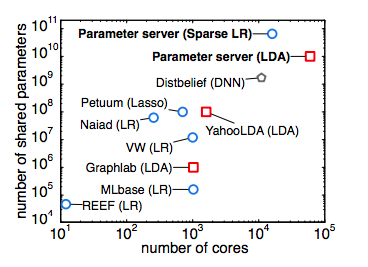
\includegraphics[width=\linewidth]{comparison_parameter_servers.png}
\caption{The comparison among large scale machine learning systems}
\label{comparison_parameter_servers}
\end{figure}

\section{Conclusion}
The conclusion goes here.





% if have a single appendix:
%\appendix[Proof of the Zonklar Equations]
% or
%\appendix  % for no appendix heading
% do not use \section anymore after \appendix, only \section*
% is possibly needed

% use appendices with more than one appendix
% then use \section to start each appendix
% you must declare a \section before using any
% \subsection or using \label (\appendices by itself
% starts a section numbered zero.)
%


\appendices
\section{Proof of the First Zonklar Equation}
Appendix one text goes here.

% you can choose not to have a title for an appendix
% if you want by leaving the argument blank
\section{}
Appendix two text goes here.


% use section* for acknowledgement
\section*{Acknowledgment}


The authors would like to thank...


% Can use something like this to put references on a page
% by themselves when using endfloat and the captionsoff option.
\ifCLASSOPTIONcaptionsoff
  \newpage
\fi



% trigger a \newpage just before the given reference
% number - used to balance the columns on the last page
% adjust value as needed - may need to be readjusted if
% the document is modified later
%\IEEEtriggeratref{8}
% The "triggered" command can be changed if desired:
%\IEEEtriggercmd{\enlargethispage{-5in}}

% references section

% can use a bibliography generated by BibTeX as a .bbl file
% BibTeX documentation can be easily obtained at:
% http://www.ctan.org/tex-archive/biblio/bibtex/contrib/doc/
% The IEEEtran BibTeX style support page is at:
% http://www.michaelshell.org/tex/ieeetran/bibtex/
%\bibliographystyle{IEEEtran}
% argument is your BibTeX string definitions and bibliography database(s)
%\bibliography{IEEEabrv,../bib/paper}
%
% <OR> manually copy in the resultant .bbl file
% set second argument of \begin to the number of references
% (used to reserve space for the reference number labels box)

\bibliography{ref}


% biography section
% 
% If you have an EPS/PDF photo (graphicx package needed) extra braces are
% needed around the contents of the optional argument to biography to prevent
% the LaTeX parser from getting confused when it sees the complicated
% \includegraphics command within an optional argument. (You could create
% your own custom macro containing the \includegraphics command to make things
% simpler here.)
%\begin{IEEEbiography}[{\includegraphics[width=1in,height=1.25in,clip,keepaspectratio]{mshell}}]{Michael Shell}
% or if you just want to reserve a space for a photo:

\begin{IEEEbiography}{Michael Shell}
Biography text here.
\end{IEEEbiography}

% if you will not have a photo at all:
\begin{IEEEbiographynophoto}{John Doe}
Biography text here.
\end{IEEEbiographynophoto}

% insert where needed to balance the two columns on the last page with
% biographies
%\newpage

\begin{IEEEbiographynophoto}{Jane Doe}
Biography text here.
\end{IEEEbiographynophoto}

% You can push biographies down or up by placing
% a \vfill before or after them. The appropriate
% use of \vfill depends on what kind of text is
% on the last page and whether or not the columns
% are being equalized.

%\vfill

% Can be used to pull up biographies so that the bottom of the last one
% is flush with the other column.
%\enlargethispage{-5in}



% that's all folks
\end{document}


